\documentclass{beamer}
\usepackage[utf8]{inputenc}
\usepackage[T1]{fontenc}
\usepackage{ragged2e}
\justifying

\newcommand{\logoWidth}{1 cm}
\newcommand{\spaceh}{0,5 cm}


 \title{Automatic exploit generation}
\author[shortname]{
Maxime Bélair  \inst{1} \and
Manh-Dung Nguyen  \inst{2} \and
Emilien Fournier \inst{3}\and
 Tristan Benoit \inst{4}\and
Gabriel Sauger \inst{5}\\
\vspace{0.3cm}
\textbf{Subject by}: \large Jules Villard - 
\includegraphics[width = 1cm]{Figures/Logos/FacebookLogo.png}
}

\institute{
\inst{1}%
Orange Labs / IMT atlantique - \tiny maxime.belair@imt-atlantique.fr
\and
\inst{2}%
CEA LIST \& Université Grenoble Alpes - \tiny manh-dung.nguyen@cea.fr
\and
\inst{3}%
ENSTA Bretagne / Lab-STICC - \tiny emilien.fournier@ensta-bretagne.org
\and
\inst{4}%
LORIA - \tiny tristan.benoit@loria.fr
\and
\inst{5}%
LORIA - \tiny gabriel.sauger@loria.fr
}
\date{}

\titlegraphic{ \vspace{-1cm}

\includegraphics[width = \logoWidth]{Figures/Logos/MaxLogo1.png}
\includegraphics[width = 0.5cm]{Figures/Logos/MaxLogo2.png}
\hspace{\spaceh}
\includegraphics[width = 0.75cm]{Figures/Logos/MDLogo1.png}
\includegraphics[width = \logoWidth]{Figures/Logos/MDLogo2.png}
\hspace{\spaceh}
\includegraphics[width = 2.5cm]{Figures/Logos/EmilienLogo1.png}
\hspace{0.5cm}
\includegraphics[width = 2CM]{Figures/Logos/GabrielLogo1.png}
\hspace{\spaceh}
}


\usetheme{Antibes}


\setbeamertemplate{footline}[frame number]


\begin{document}

\begin{frame}
\titlepage
\end{frame}


\section{Problem overview}

\begin{frame}
\centering
\LARGE
Problem Overview
\end{frame}

\subsection{Context}

\begin{frame}{Context}

\begin{itemize}
\item Bugs in devices
\item Are they weaknesses ?
\end{itemize}

\begin{figure}
\includegraphics[width = 2cm]{Figures/HeartbleedLogo.png}
\end{figure}

\begin{block}{Formal challenge}
Can we automatically turn static analysis reports into executable confirming the vulnerability of a program ?
\end{block}


\end{frame}

\subsection*{Section example}
\begin{frame}{Section example}
\textit{Give an example of main.c with a bug}
We can show pictures or live performance. Ask the audience to detect the bug.
\end{frame}

\subsection{Infer tool}

\begin{frame}{Infer tool}

\begin{figure}
\includegraphics[width=10cm]{Figures/InferDrawing.png}
\end{figure}

\end{frame}

\begin{frame}

\begin{figure}
\includegraphics[width = 1.8cm]{Figures/InferLogo.png}

\end{figure}

\vspace{1cm}

\begin{itemize}
\item Static analysis tool from Facebook
\item \textbf{Capture} phase, then \textbf{Analysis} phase
\end{itemize}

\end{frame}

\begin{frame}{Infer tool example}

\textit{Give an example of our use of Infer on main.c}
We can show pictures or live performance.
\end{frame}

\subsection{Practical approach}

\begin{frame}{Practical approach}

\begin{figure}
\includegraphics[width=9.5cm]{Figures/Workflow.png}
\end{figure}

\end{frame}


\begin{frame}{Practical approach}

\begin{block}{Practical challenge}
Given the Infer information about bugs of a program A, create a program B that crashes A
\end{block}

\end{frame}

\begin{frame}{Table of content}
\tableofcontents
\end{frame}

\section{Proposed approaches}

\begin{frame}
\centering

P\LARGE roposed approaches
\end{frame}



\subsection{Model checking}

\begin{frame}{Model checking}

Present model checking solution with Divine

\end{frame}


\subsection{SMT solvers}

\begin{frame}{SMT solvers}

Present logic solvers

\end{frame}

\begin{frame}{SMT Solvers}
Compiler / Interpreter information
\end{frame}

\begin{frame}{SMT Solver}
\includegraphics[width=9cm]{Figures/SMTsolver/SMTsolverCompete.png}
\end{frame}

\begin{frame}{SMT results}
Present the results we have and on which program. The performance review is NOT done here, but in Part 3/Result Comparison
\end{frame}

\subsection{Fuzzing technique}

\begin{frame}{Fuzzing technique}

Present fuzzing techniques

\end{frame}

\begin{frame}{Fuzzing technique}

\begin{figure}
\includegraphics[width=10cm]{Figures/Fuzzing.png}
\end{figure}

\end{frame}


\section{Conclusions and perspectives}

\begin{frame}
\centering
\LARGE Conclusions and perspectives
\end{frame}

\subsection{Results comparison}

\begin{frame}{Results comparison}

\textit{Show a table approaches / program comparing results (yes/no, running time, implementation complexity, computational complexity } \\

\end{frame}

\subsection{Future Work}
\begin{frame}{Future work}

Put eeeeeverything we think of. Ex:

\begin{itemize}
\item Generate 
\item Create a fully automatic process
\item Find automatic ways to generate exploits (using dictionary like attacks)
\end{itemize}

\end{frame}


\begin{frame}{Thank you Questions ?}

See the title

\end{frame}

\end{document}
